%--------------------------------------------------------------
% thesis.tex 
%--------------------------------------------------------------
% Corso di Laurea in Informatica 
% http://if.dsi.unifi.it/
% @Facolt\`a di Scienze Matematiche, Fisiche e Naturali
% @Universit\`a degli Studi di Firenze
%--------------------------------------------------------------
% - template for the main file of Informatica@Unifi Thesis 
% - based on Classic Thesis Style Copyright (C) 2008 
%   Andr\'e Miede http://www.miede.de   
%--------------------------------------------------------------
\documentclass[twoside,openright,titlepage,fleqn,
	headinclude,12pt,a4paper,BCOR5mm,footinclude]{scrbook}
%--------------------------------------------------------------
\newcommand{\myItalianTitle}{Utilizzo di Soft-Brownian-Offset per la generazione di attacchi ai fini dell’addestramento di rilevatori di intrusioni\xspace}
\newcommand{\myEnglishTitle}{Application of Soft-Brownian-Offset to generate cyber-attacks to train intrusion detectors\xspace}
\newcommand{\myDegree}{Corso di Laurea in Informatica\xspace}

\newcommand{\tablelegend}[1]{\centering\textbf{#1}}


%\newcommand{\myDegree}{
	%Corso di Laurea Specialistica in Scienze e Tecnologie
	%dell'Informazione\xspace}

\newcommand{\myName}{Guglielmo Bartelloni\xspace}
\newcommand{\myProf}{Andrea Ceccarelli\xspace}
\newcommand{\myOtherProf}{Correlatore\xspace}
\newcommand{\mySupervisor}{Andrea Ceccarelli\xspace}
\newcommand{\myFaculty}{
	Scuola di Scienze Matematiche, Fisiche e Naturali\xspace}
\newcommand{\myUni}{\protect{
	Universit\`a degli Studi di Firenze}\xspace}
\newcommand{\myLocation}{Firenze\xspace}
\newcommand{\myTime}{Anno Accademico 2022-2023\xspace}
\newcommand{\myVersion}{Version 0.1\xspace}
%--------------------------------------------------------------
\usepackage[italian]{babel}
\usepackage[utf8]{inputenc} 
\usepackage[T1]{fontenc} 
\usepackage[square,numbers]{natbib} 
\usepackage{amsmath}  
\usepackage{ellipsis}
\usepackage{listings}
\usepackage{subfig}
\usepackage{caption}
\usepackage{appendix}
\usepackage{siunitx}
\usepackage{natbib}
\usepackage{pythonhighlight}

%--------------------------------------------------------------
\usepackage{dia-classicthesis-ldpkg}
%\usepackage{classicthesis}
%--------------------------------------------------------------
% Options for classicthesis.sty:
% tocaligned eulerchapternumbers drafting linedheaders 
% listsseparated subfig nochapters beramono eulermath parts 
% minionpro pdfspacing
\usepackage[eulerchapternumbers,linedheaders,subfig,beramono,eulermath,
parts]{classicthesis}

\usepackage{lmodern} 
\usepackage{diagbox}
%--------------------------------------------------------------
\newlength{\abcd} % for ab..z string length calculation
% how all the floats will be aligned
\newcommand{\myfloatalign}{\centering} 
\setlength{\extrarowheight}{3pt} % increase table row height
\captionsetup{format=hang,font=small}
%--------------------------------------------------------------
% Layout setting
%--------------------------------------------------------------
\usepackage{geometry}
\geometry{
	a4paper,
	ignoremp,
	bindingoffset = 1cm, 
	textwidth     = 13.5cm,
	textheight    = 21.5cm,
	lmargin       = 3.5cm, % left margin
	tmargin       = 4cm    % top margin 
}

\lstset{
  	frame=tb,
	language=Matlab,
  	aboveskip=3mm,
  	belowskip=3mm,
  	showstringspaces=false,
  	columns=flexible,
  	basicstyle={\small\ttfamily},
  	numbers=none,
  	breaklines=true,
  	breakatwhitespace=true,
  	tabsize=3
}
%--------------------------------------------------------------
\begin{document}
\frenchspacing
\raggedbottom
\pagenumbering{roman}
\pagestyle{plain}
%--------------------------------------------------------------
% Frontmatter
%--------------------------------------------------------------
%--------------------------------------------------------------
% titlepage.tex (use thesis.tex as main file)
%--------------------------------------------------------------
\begin{titlepage}
	\begin{center}
   	\large
      \hfill
      \vfill
      \begingroup
         
\includegraphics[scale=0.15]{logo/LOGO}\\
%			\spacedallcaps{\myUni} \\ 
			\myFaculty \\
			\myDegree \\ 
			\vspace{0.5cm}
         \vspace{0.5cm}    
         Tesi di Laurea    
      \endgroup 
      \vfill 
      \begingroup
      	\color{Maroon}\spacedallcaps{\myItalianTitle} \\ $\ $\\
      	\spacedallcaps{\myEnglishTitle} \\ 	
	\bigskip
      \endgroup
      \spacedlowsmallcaps{\myName}
      \vfill 
      \vfill
      Relatore: \emph{Relatore}\\
      Correlatore: \emph{Correlatore}\\
      \vfill
      \vfill
      \myTime
      \vfill                      
	\end{center}        
\end{titlepage}   
%--------------------------------------------------------------
% back titlepage
%--------------------------------------------------------------
   \newpage
	\thispagestyle{empty}
	\hfill
	\vfill
	\noindent\myName: 
	\textit{\myItalianTitle,} 
	\myDegree, \textcopyright\ \myTime
%--------------------------------------------------------------
% back titlepage end
%--------------------------------------------------------------
\pagestyle{scrheadings}
%--------------------------------------------------------------
% Mainmatter
%--------------------------------------------------------------
\pagenumbering{arabic}
% use \cleardoublepage here to avoid problems with pdfbookmark
%\include{intro} % use \myChapter command instead of \chapter
\tableofcontents
\listoffigures
\cleardoublepage
\thispagestyle{empty}
\begin{flushright}
\null\vspace{\stretch {1}}
\emph{"If you put water into a cup, it becomes the cup. You put water into a bottle, it becomes the bottle. You put it in a teapot, it becomes the teapot. Now, water can flow or it can crash. Be water, my friend." \break --- Bruce Lee} \vspace{\stretch{2}}\null
\end{flushright}
\cleardoublepage
\include{Chapters/Introduzione}
\include{Chapters/Fondamenti}
\chapter{Soft Brownian Offset}

Soft Brownian Offset (SBO) è un algoritmo per la generazione di dati sintetici fuori dalla distribuzione (Out of Distribution OOD). 

È stato sviluppato da ~\cite{sbo} inizialmente per poter migliorare il rilevamento dei dati fuori dalla distribuzione, si pensi ad esempio nel caso dei cyber-physical systems (CPS) e.g. auto a guida autonoma, dove il rilevamento di eventi anomali è di vitale importanza ~\cite{yuhasEmbeddedOutofdistributionDetection2021}.

Per questo scopo i dati generati necessitano di essere non troppo dissimili da quelli originali, perché altrimenti il modello potrebbe soffrire di "overconfidence" ~\cite{amodeiConcreteProblemsAI2016}.

SBO si basa sul "Gaussian Hyperspheric Offset" che cerca di creare i dati OOD campionando attraverso una ipersfera attorno ai dati iniziali (In Distribution).

Partendo da quest'ultimo algoritmo, SBO permette di utilizzare qualsiasi punto del dataset e traslarlo in modo da avere una certa distanza minima dagli altri punti. I dati vengono processati da un autoencoder (AE) addestrato su un particolare dataset. La figura \ref{fig:sbo_schema} mostra graficamente questo approccio. 


\begin{figure}[htpb]
    \centering
    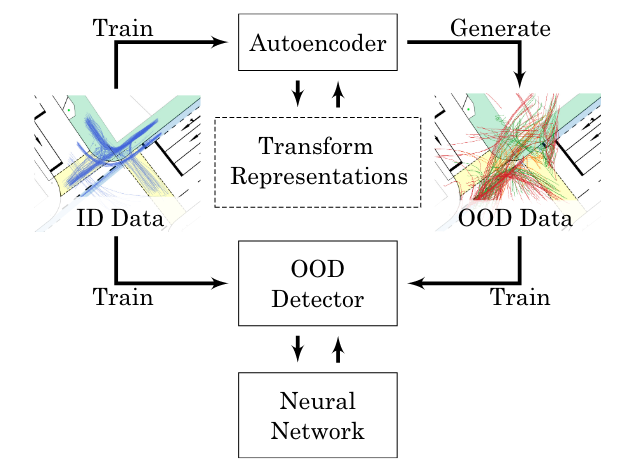
\includegraphics[width=\textwidth,height=10cm,keepaspectratio=true]{img/sbo_schema.png}
    \caption{
        Schema che rappresenta l'approccio utilizzato da SBO. Inizialmente i dati ID vengono usati per addestrare l'autoencoder e successivamente vengono generati i dati OOD tramite SBO. Questi poi vengono decodificati dall'AE per integrarsi nel dataset iniziale. Infine, viene addestrata una rete neurale, nel nostro caso invece, utilizzeremo XGBoost.
    }
    \label{fig:sbo_schema}
\end{figure}


\section{Autoencoder} 

Un autoencoder è una particolare rete neurale che ha il compito di codificare un input e comprimerlo in una rappresentazione rilevamente per poi decodificarlo e ricostruirlo nel modo più fedele possibile ~\cite{bankAutoencoders2021}.

Il loro compito principale è quindi di imparare, in modo non supervisionato, una rappresentazione ridotta significativa dei dati.

Il problema può essere formalmente definito ~\cite{baldiAutoencodersUnsupervisedLearning}, come trovare le funzioni $A$:$ R^{n} \rightarrow R^p$ (encoder) e $B$:$ R^{p} \rightarrow R^n$ (decoder) in modo che:

\begin{center}
$arg min_{A,B} E$[$\Delta$($x,  B$($A$($x$)))] \\
\end{center}

dove $E$ è la distribuzione di $x$ che ci si aspetta, e $\Delta$ è la funzione obbiettivo della ricostruzione, che misura la distanza tra l'output del decoder e l'input.

La figura \ref{fig:ae_schema} mostra il processo del modello autoencoder.

\begin{figure}[htpb]
    \centering
    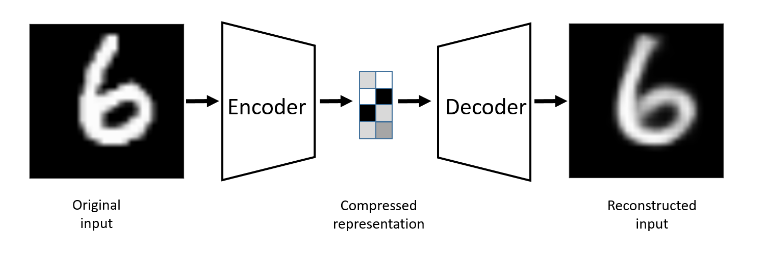
\includegraphics[width=\textwidth,height=10cm,keepaspectratio=true]{img/ae_schema.png}
    \caption{
        Schema che rappresenta il modello autoencoder. Da ~\cite{baldiAutoencodersUnsupervisedLearning}
    }
    \label{fig:ae_schema}
\end{figure}


L'approccio utilizzato per Soft Brownian Offset è quello di addestrare un autoencoder sul dataset di partenza, ridurre lo spazio di lavoro utilizzando l'encoder, generare i dati OOD ed infine ricostruire il dataset attraverso il decoder.



\chapter{Generazione di attacchi usando Soft Brownian Offset}
\label{chap:generazione_di_attacchi_usando_sbo}

Parleremo inizialmente del processo di preparazione ed analisi dei dati, di come è stato utilizzato Soft Brownian Offset ed infine verranno illustrati i metodi di calcolo dell'accuratezza del modello.

Nel capitolo successivo verranno mostrati i risultati ottenuti.


\section{Metodologie}

Ogni dataset è stato analizzato, per capire quali fossero i dati più significativi per l'addestramento del modello. 

È stato necessario filtrare alcune colonne che contenevano valori non numerici come, nel caso di CIC-IDS, la colonna "Timestamp" che includeva la data e l'ora del pacchetto. 

Inoltre le righe contenenti valori come "Inf" o "NaN" sono state modificate perché, se lasciate intatte, avrebbero causato errori durante la generazione dei dati out-of-distribution.

Entrambi i dataset hanno una colonna "label" per indicare la tipologia del pacchetto, nello specifico, sono presenti le tipologie varie tipologie di attacchi e.g. "bruteForce", "dos", "pingScan", "portScan". Dato che, nel nostro caso, non ci interessa sapere nello specifico l'attacco del pacchetto, tutti gli attacchi, sono stati etichettati come "attack".

Dopo aver fatto queste operazione di preprocessamento, si è passati alla generazione dei sample OOD.

La prima prova effettuata è stata quella di utilizzare Soft Brownian Offset a partire dal dataset completo senza distinzioni di tipologia di pacchetto, per vedere se era possibile in questo modo, generare degli attacchi verosimili. Questa soluzione però genera dei pacchetti che sono troppo vicini, in termini di caratteristiche, a quelli normali perché i dataset hanno una quantità molto maggiore di dati normali rispetto a quelli di attacchi. Abbiamo quindi dovuto scartare questo metodo.

Un altro metodo possibile che non è stato approfondito è quello di generare i pacchetti come sopra, filtrando i pacchetti troppo "vicini" (sempre in termini di caratteristiche) ai pacchetti normali. Si ottiene così un dataset che ha la giusta quantità di dati out-of-distribution e potrebbe migliorare l'apprendimento di un modello.

Il metodo che invece abbiamo utilizzato e che  ottiene risultati buoni risultati è quello di utilizzare Soft Brownian Offset solo sui pacchetti di attacco, in questo modo si ottiene delle varianti dei pacchetti di attacco che riescono a migliorare il rilevamento da parte degli IDS.

Confronteremo inoltre i risultati con una generazione di pacchetti effettuata a partire da solo traffico normale evidenziando le differenze che si hanno con i due approcci.

Per il calcolo delle performance del modello XGBoost, a seguito dell'addestramento, si è utilizzato il coefficiente di Matthews.



% \subsection{Analisi dei dati iniziali}
%
%
% \subsection{Generazione dei pacchetti}
%
% \subsection{Addestramento del modello}
%
% \subsection{Metriche utilizzate}
%
% \subsubsection{Accuracy}
%
% \subsubsection{Metthews}
%

\include{Chapters/Risultati}
\include{Chapters/Conclusioni}
\bibliographystyle{ieeetr}
\bibliography{biblio}
%--------------------------------------------------------------
\end{document}
%--------------------------------------------------------------
